\chapter{Differential characterisation of disulfide bonds}\label{chap:methods}

% TODO Přidat krátkou sekci o nastavení, která jsme používali k analýze

\paragraph{Reagents and instrumentation} Trypsin was purchased from Roche, lysosyme and lipase were obtained from Sigma-Aldrich. The used liquid chromatography setup was RSLC nano Ultimate 3000 (Thermo Scientific), for tandem mass spectrometry Orbitrap Fusion Lumos (Thermo Scientific) was employed.

\paragraph{Obtaining the data} We have anaylzed two proteins, lysosyme (LYS) and lipase (LIP). Two samples of each have been obtained in separate sample preparation pathways; in the AT sample preparation pathway, the samples have been alkylated without prior reduction, while in the RAT pathway, reduction took place before the alkylation. In both cases the alkylation has been done by iodacetamide (IAA), resulting in a covalent addition of a carbamidomethyl group (57.07 Da) onto cysteines without DBs; the reduction was achieved by dithiothreitol (DTT). After that, all four samples have been fully digested by trypsine, resulting in two sets of tryptides for each of the two analysed proteins. The samples have been treated the same for the rest of the experiment. After digestion, the peptides had undergone reverse-LC separation that was directly connected to the mass spectrometer through a nanospray ion source. After the measurement of MS\textsuperscript{1} spectra on a quadrupole, the precursors continue on to be fragmented with HCD\@. The MS\textsuperscript{2} spectra were analysed on an orbitrap analyser, as is implied by the use of HCD fragmentation. Finally, raw MS\textsuperscript{2} match data was exported to mgf files. Additionaly an artifical testing dataset based on in-silico digestion and fragmentation of he protein ovalbun has been prepared.

The data have been kindly provided by a IOCB mass specrometry research group (J. Cvačka), and have been measured a few years ago without any direct connection to this thesis.

\section{Dibbi, a program for DB visualisation}

We have developed a command-line Python program called Dibbi that aims to automatically determine the positions of DBs in a protein. Its input is the sequence of the analysed protein, and the mgf file with the measured MS\textsuperscript{2} data. After many processing steps, Dibbi creates a visualisation of evidence for each possible DB, and produces a file with the processed data, allowing for further manual analysis of the results should the user so desire. Dibbi is able to operate even if only data from AT samples are provided, but to obtain the best results it is preferable to do a differential analysis based on data from RAT samples.

Dibbi's main wofklow is split into two separate stages: match assignment, and evidence scoring and visualisation. Both of them are described in detail in their separate sections, what follows is a brief summary. The first stage can be further broken down into discrete steps that are illustrated on \Cref{fig:pipeline}, and listed below.

\begin{enumerate}
	\item Dynamically generated \emph{precursors} are assigned to the precursor masses from the input. The result of this stage is a list of \emph{precursors}, which are effectively slices of the input protein with an added information about the number of DBs and amino acid modifications.
	\item \emph{Variants} are generated from the precursor; a variant is also a slice of the original protein, but with concretely specified configuration of DBs and alkylations. The more cysteines and DBs there are in a precursor, the more variants are generated from it, becuase a variant is generated for every valid combination of bonds and alkylations.
	\item \emph{Fragments} produced from the variants are assigned to peaks from the respective spectra.
\end{enumerate}

The second stage interprets the data generated by the first stage; the steps are briefly summarised on \Cref{fig:score-calculation}, and can be descibed as:

\begin{enumerate}
	\item Precursor assignments are scored, based on their various properties.
	\item Fragment assignemnts are scored, again based on their various properties.
	\item Variants are scored by combining the score of their parent precursor and the scores of their fragments.
	\item The evidence about individual DBs or alkylated cysteines being present in a fragment is weighted by the score of the variant of the fragment, then the evidence from all fragments is aggregated and the results are visualised.
\end{enumerate}


\begin{figure}
	\centering
	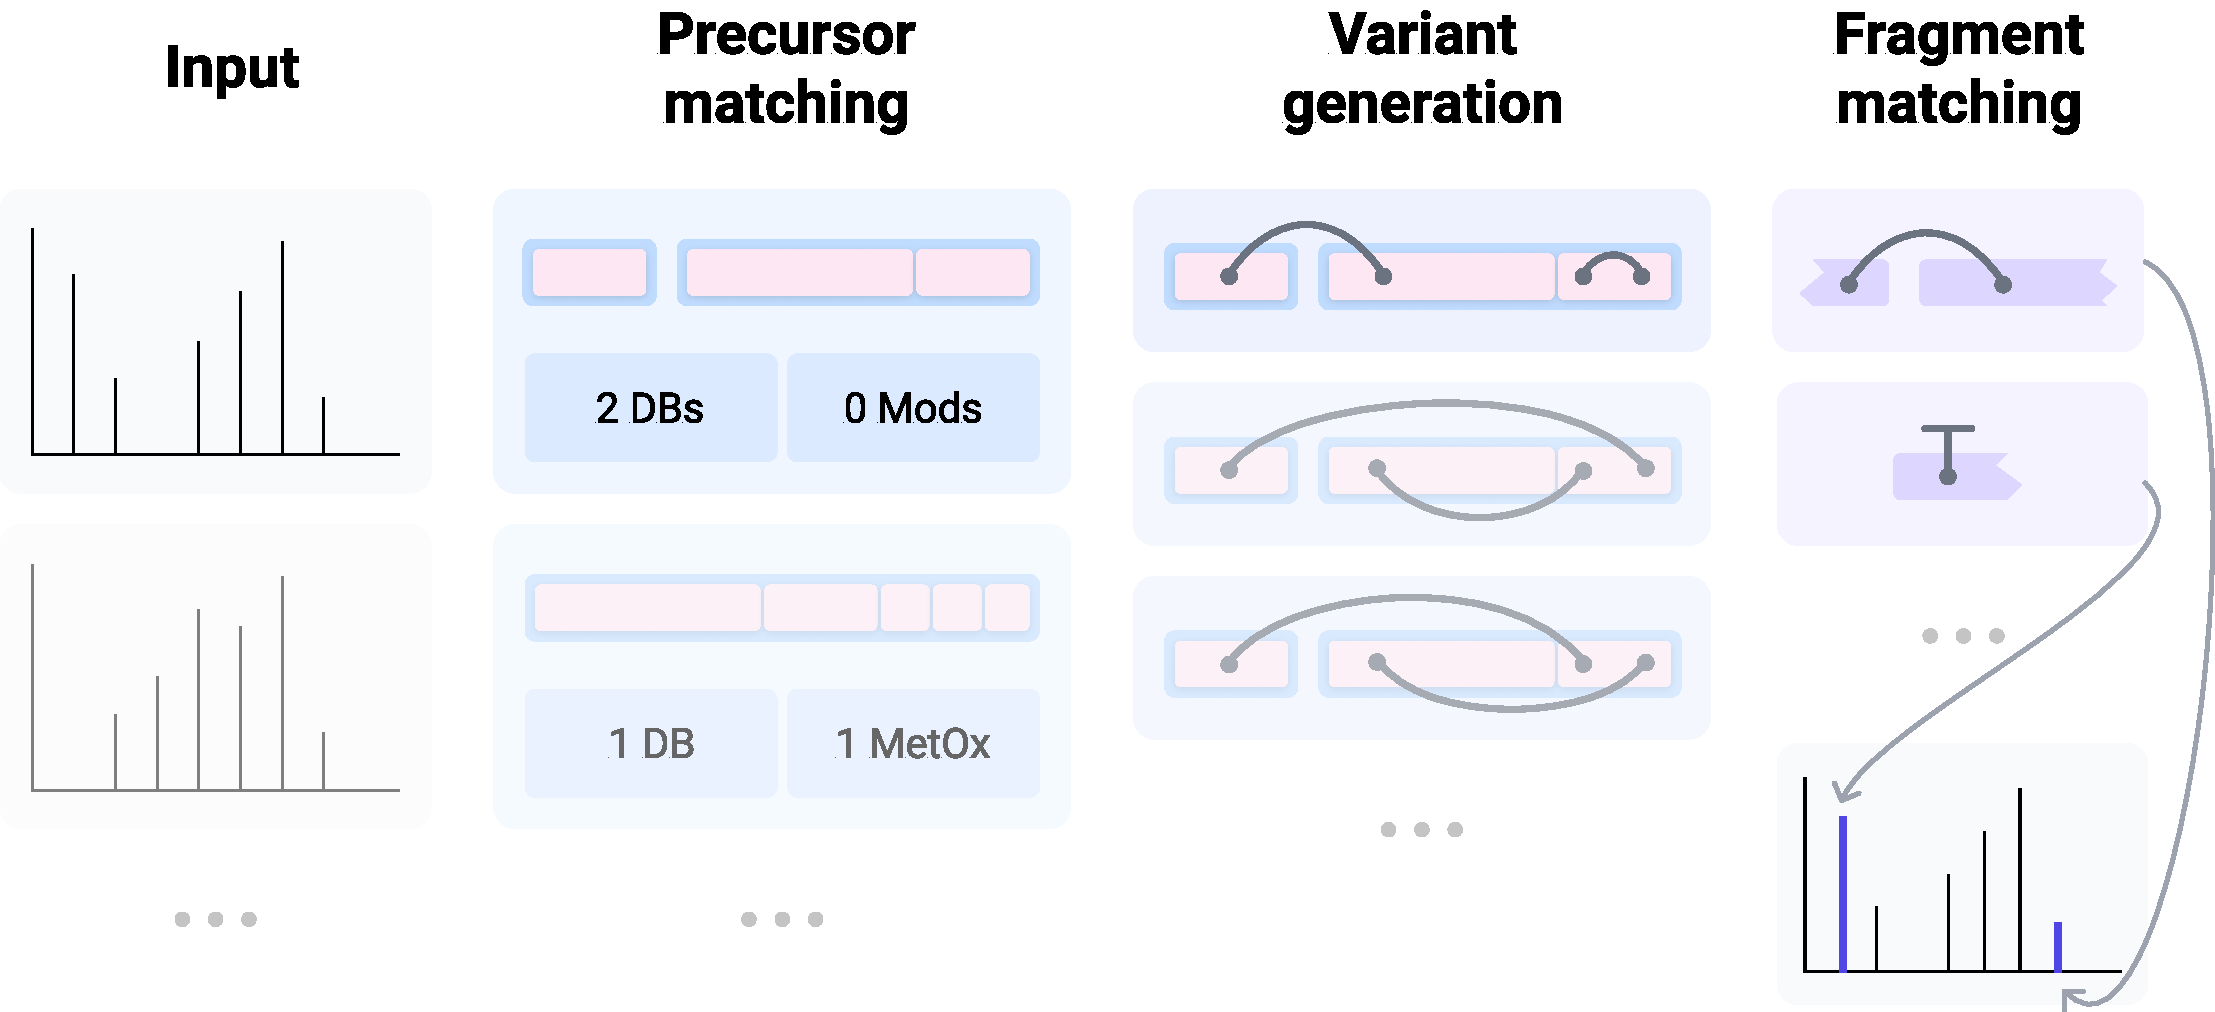
\includegraphics[width=\linewidth]{img/pipeline.pdf}
	\caption{The processing and assignment pipeline in Dibbi, not including scoring and visualisation. First, precursors are assigned to the provided spectra, then the precursors are used to generate \emph{variants}, and finally, fragments of the variants are assigned to the peaks in the spectra. Refer to the main text for definitions of each of the terms. Pink bits represent basal peptides resulting from protein digestion, or \emph{tryptides}, and the bigger blue rectangles around them respresent \emph{segments}, longer peptides made of one or more \emph{tryptides}.}\label{fig:pipeline}

\end{figure}

\begin{figure}
	\centering
	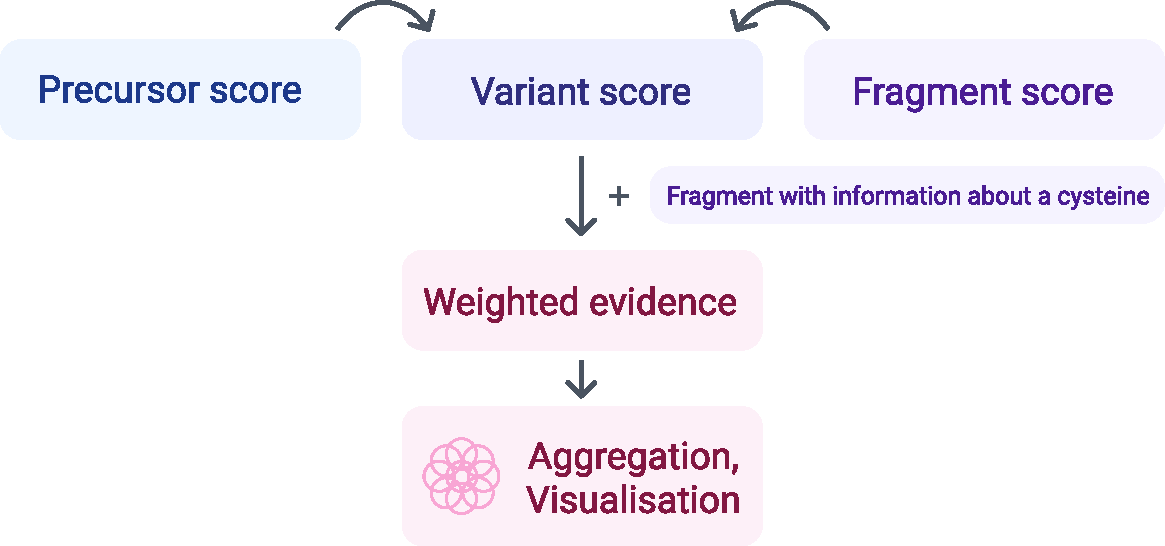
\includegraphics[width=0.9\linewidth]{img/score-calculation.pdf}
	\caption{Our goal is to evalute the evidence for each possible disulfide bond; the evidence is gathered from the fragment assignments. To forster the quality of the evidence, Dibby tries to weed out false positive assignments by weighting evidence from each fragment by the score of its variant. The variant score is calculated from the precursor score and the score of assigned fragments belonging to the variant.}\label{fig:score-calculation}
\end{figure}


\subsection{Precursor assignment}

At the beginning, the protein undergoes a complete in-silico digestion, producting basal peptides that can not be digested any further; the protease of our choosing was trypsin, so we call these basal peptides \emph{tryptides}. As mentioned in the first chapter (\Cref{sec:trypsin}), a protease can sometimes miss a cleavage point, resulting in a peptie chain that is made from two (or more) contiguous basal tryptides. We call a chain of one or more tryptides a \emph{segment}, altough it is technically only a plain peptide, just as the tryptides are. Due to the crosslinking by DBs in our samples, a \emph{precursor} is made out of one or more segments connected with interpeptide disulfide bonds\footnote{There can be one or more DB connecting a segment to another segment, and there can also be intrasegment DBs.}.


From the point of view of this part of the algorithm, it matters not where the individual DBs are located, because the individual \emph{variants} are not distiguishable on the basis of precursor mass. Thus, for each precursor that it managed to assign to a spectrum, the output of the algorithm only includes the following information:

\begin{itemize}
	\item  Which segments are present in the precursor.
	\item How many DBs there are in the precursor.\footnote{The number of DBs is always at least the number of segments minus 1.}, and, by extension, how many alkylated cysteines there are --- every cysteine that does not partake in a bond is considered alkylated. Notice the algorithm does not say anything about \emph{where} the bonds or alkylations are.
	\item How many other amino acid modifications, for example methionine oxidations, are there? The set of available modifications is configurable, and these modifictaions are treated the same as ``variable'' modifications are treated in other software,
\end{itemize}


The precursor is built iteratively segment by segment, and the individual segments are built tryptide by tryptide, every time from left to right. First of all, given a target mass to which we want to assign a precursor, the algorithm chooses a beginning of the first segment. After that the \textsc{FindPrec} function iteratively branches out to search the solution space for precursors with a theoretical mass within an error boundary around the target mass. In each iteration, the following branching points are tried out:

\begin{enumerate}
	\item Combine the possible modifications and DBs in such a way that the \Var{Selected} segments with the modifications have the correct mass, using the \textsc{Combine} function (see \algref{alg:findprec}{alg:findprec:combinations}). \textsc{Combine} implements a divide-and-conquer algorithm for a modified subset sum problem, in which assignments that are within some error boundary of the target are also considered a valid solution.
	\item Elongate the current segment by adding the current tryptide to it (see \algref{alg:findprec}{alg:findprec:elongate}, and also the whole \Cref{alg:elongate}).
	\item End the current segment (effectively simulating a protease cleavage just before the current tryptide) and begin a new one that begins on the current tryptide or later. See \algref{alg:findprec}{alg:findprec:end}, and the whole \Cref{alg:newseg}.
\end{enumerate}

The fact taht the precursors (and their segments) are built strictly from left to right is a simple form of symmetry breaking --- that is, not generating the multiple equivalent symmetrical solutions. Some further optimizations were added as well, mainly to prevent traversing a branch once we learn it can not provide any more solutions. The used protease is configurable, as well as the amino acid modifications and the maximum number of segments we want the found precursors to have.

% TODO Zkrátit algoritmy na základní myšlenku, a la fragmenty


\begin{algorithm}
	\begin{algorithmic}
		\Function{FindPrec}{$I, \mathit{Selected}, \mathit{Mass}, \mathit{Segments}, \mathit{Cys}, \mathit{Open}$}
		\State $\mathit{solutions} \gets$ empty list

		\nb{There is no hanging disulfide bond from previous segments}
		\nb{So let us try to combine residue modifications to find a solution}
		\If{not $\mathit{Open}$}\label{alg:findprec:combinations}
		\State $mods \gets$ calculate possible modifications from $\mathit{Selected}$
		\State $alks \gets$ calculate alkylation count based on seen non-bonded $\mathit{Cys}$
		\State $combinations \gets$ \Call{Combine}{$mass, mods, alks$}
		\State return a list of precursors generated from $combinations$
		\EndIf

		\nb{There are no further solutions, our $\mathit{Mass}$ can not get low enough}
		\If{$\mathit{Mass}$ is too high, or $i$ is at the end}
		\State return empty list
		\EndIf

		\nb{End this segment, connect next one with a disulfide bond}
		\nb{That is, if we have the segments budget and a free cysteine}
		\If{not $\mathit{Open}$, and $\mathit{Segments} > 0$, and $\mathit{Cys} > 0$}\label{alg:findprec:end}
		\State $S \gets$ \Call{NewSegment}{$I, \mathit{Selected}, \mathit{Mass}, \mathit{Segments}, \mathit{Cys}, \mathit{Open}$}
		\State concatenate $\mathit{solutions}$ with the list $S$
		\EndIf

		\nb{Elongate the current segment by one tryptide}
		\State $S \gets$ \Call{Elongate}{$I, \mathit{Selected}, \mathit{Mass}, \mathit{Segments}, \mathit{Cys}, \mathit{Open}$}\label{alg:findprec:elongate}
		\State concatenate $\mathit{solutions}$ with the list $S$
		\State return the list $\mathit{solutions}$

		\EndFunction
	\end{algorithmic}
	\caption{The main part of the precursor matching algorithm, in which all the braching occurs.}\label{alg:findprec}
\end{algorithm}


\begin{algorithm}
	\begin{algorithmic}
		\Function{Elongate}{$I, Selected, \mathit{Mass}, \mathit{Segments}, \mathit{Cys}, \mathit{Open}$}
		\nb{Prolong the current segment by one tryptide}

		\State $\mathit{tryptide} \gets$ the $I$-th tryptide from the list $\mathit{TRYPTIDES}$
		\State $\mathit{mass'} \gets$ the mass of $\mathit{tryptide}$ added to $\mathit{Mass}$
		\State $\mathit{cys'}\gets$ the number of cys in $\mathit{tryptide}$ added to $\mathit{Cys}$
		\Decl{cys'}{lower \Var{cys'} by one if \Var{Open} is true, using a cys to close the bond}
		\State $\mathit{open'} \gets$ False if this tryptide had any cysteines, otherwise $\mathit{Open}$

		\nb{Call the original function}
		\State $S \gets$ \Call{FindPrec}{$I + 1, \mathit{Selected}, \mathit{mass'}, \mathit{Segments}, cys', \mathit{open'}$}
		\State return the list $S$

		\EndFunction
	\end{algorithmic}
	\caption{Elongates the currently built precursor segment, adding the current tryptide to it.}\label{alg:elongate}
\end{algorithm}


\begin{algorithm}
	\begin{algorithmic}
		\Function{NewSegment}{$I, \mathit{Selected}, \mathit{Mass}, \mathit{Segments}, \mathit{Cys}, \mathit{Open}$}
		\State $sel' \gets$ the currently ending segment added to $\mathit{Selected}$
		\State $\mathit{mass'} \gets$ subtract mass of $\ce{H2}$ from $\mathit{Mass}$, due to the new DB
		\nb{Update the budget, because of the newly started segment}
		\State $\mathit{seg'} \gets \mathit{Segments} - 1$
		\nb{Begin the bond with one of our cysteines}
		\State $\mathit{cys'}\gets \mathit{Cys} - 1$
		\nb{The new bond is waiting to get ``closed'' by a cys in the next run}
		\State $\mathit{open'} \gets$ True

		\nb{Finally, branch out: start a new segment from all possible starting points}
		\For{all possible beginings of the next segment from $I + 1$ onward}
		\State $i' \gets$ the next beginning
		\State $S \gets$ \Call{FindPrec}{$\mathit{i'}, \mathit{selected'}, \mathit{mass'}, \mathit{segments'}, \mathit{cys'}, \mathit{open'}$}
		\State return the list $S$
		\EndFor

		\EndFunction
	\end{algorithmic}
	\caption{Ends the currently built precursor segment and begins a new one, beginning with the current tryptide, or any tryptide coming after it.}\label{alg:newseg}
\end{algorithm}


\subsection{Assigning fragment mass}

Our task now is to assign in-silico generated precursor fragments to the peaks from the spectra. The quality of these assignments will later be used to score the precursor matches and ultimately to find out some information about the position of DBs in the protein.

Before the main of this stage of the program, there is an in-between processing step that takes a precursor from the precursor-matching stage, and generates all possible \emph{variants} it could represent. A \emph{variant} is a set of segments with precisely defined DB crosslinks --- that differentiates it from a precursor (which is the output of the previous stage), as precursor only holds information about the number of DBs, but not their positions.

Similarly to how precursors are constructed from crosslinked segments, and the segments from basal tryptides, fragments can also be broken down to smaller pieces; we call them \emph{cuts}. A \emph{cut} is a part of a precursor segment; it never spanns more than one segment. All of the fragment cuts form a connected subgraph in the variant graph.

A rough outline of the algorithm can be seen in \Cref{alg:fragment}. At the start, a beginning is chosen for the first cut of the fragment. In further iterations of the main function, the algorithm branches out. Before we describe the braching, we have to explain the notion of \emph{pivots}. Imagine the algorithm is building a cut, residue by residue, and it encouters a cysteine connected with a DB to another segment in the variant. When the algorihm makes the decision to keep the bond intact, the other cysteine surely will have to be in the final fragment, possibly with some other neighbouring residues from its segment. The cysteine is thus added to the list of \emph{pivots}, and when the current cut is ended, the algorithm jumps to the next pivot from the list and builds a new cut around them.

In this way, the algorithm can jump back and forth between segments, following the directions of DBs in the variant, building cuts around cysteines, until it runs out of pivots, runs out of residues in the variant, or until its mass is too high. The algorithm keeps track of all residues that are part of the current fragment, in order not to add any residue twice by adding cuts with nonempty intersection. Furthermore, the number of peptide bond and disulfide bond breaks is bounded, usually to be at most 1 or 2.

In each iteration, the algorithm attempts to do all of the following:

\begin{enumerate}
	\item Try to combine the masses of the selected cuts and some of the variable modifications to obtain a fragment with a mass that is within the error boundary around the target mass. In case of a success, add this fragment (that is, this combination of cuts and modifications) to a list of solutions.
	\item If the current residue is a cysteine partaking in a DB that we have not seen yet, branch out. Break the bond in one branch, adding assymetric modifications to both of the cysteines, and keep the bond intact in the other, adding a new \emph{pivot} to the list of pivots.
	\item Elongate the current cut by adding the next residue to it. The ``next residue'' is simply the next residue in the segment from which the cut is made. If there is no ``next residue'' in this segment, end this cut, and jump to the next pivot. If there is no pivot to jump to, end this branch of the algorithm.
	\item End this cut prematurely (in the middle of a segment), that is, simulate a peptide bond dissociation in the precursor. Jump to the next pivot, if there is any, or end this branch of the algorithm.
\end{enumerate}


\begin{algorithm}
	\begin{algorithmic}
		\Function{FragFind}{$I, \mathit{BreaksLeft}, \mathit{ValidEndRange}, \mathit{Mass}, \mathit{Pivots}$}

		\Decl{solutions}{an empty list}

		\Decl{can end}{the end would not be premature, or \Var{BreaksLeft} $> 0$}
		\If{\Var{I} is in \Var{ValidEndRange}, and also \Var{can end}}

		\If{can \textsc{Combine} the cuts with some mods to match \Var{TARGET}}
		\Decl{solutions}{the current \Var{solutions} with any of the new ones added}
		\EndIf

		\If{there is some pivot $\mathit{p}$ in $\mathit{Pivots}$}
		\Decl{startrange, endrange}{the valid cut range around \Var{p}}
		\Decl{pivots'}{\Var{pivots} with the pivot \Var{p} removed}
		\Decl{breaks'}{\Var{BreaksLeft}, possibly one less if the end is premature}
		\For{every valid cut start in \Var{startrange}}
		\Decl{S}{\Call{FragFind}{$\mathit{start}, \mathit{breaks'}, \mathit{endrange}, \mathit{Mass}, \mathit{pivots}$}}
		\Decl{solutions}{the current \Var{solutions} concatenated to \Var{S}}
		\EndFor
		\EndIf

		\EndIf

		\If{the \Var{I}-th residue is a cys partaking in a DB we have not seen yet}

		\nb{Break the bond...}
		\If{we have some breaks to spare}
		\State add the current cysteine to the broken bond counter, then...
		\Decl{mass'}{the current \Var{Mass} added to the mass of the \Var{I}-th residue}
		\Decl{S}{\Call{FragFind}{$I + 1, \mathit{BreaksLeft} - 1, \mathit{ValidCutRange}, \mathit{mass'}, \mathit{pivots}$}}
		\Decl{solutions}{the current \Var{solutions} concatenated to \Var{S}}
		\EndIf
		\nb{...or keep it intact}
		\Decl{pivots'}{add the other end of the bond to \Var{Pivots}}
		\Decl{mass'}{the mass of the bond, $\ce{H2}$, subtracted from \Var{Mass}}
		\Decl{S}{\Call{FragFind}{$I + 1, \mathit{BreaksLeft}, \mathit{ValidCutRange}, \mathit{mass'}, \mathit{pivots'}$}}

		\Decl{solutions}{the current \Var{solutions} concatenated to \Var{S}}

		\Else
		\nb{Continue adding to this cut}
		\Decl{mass'}{the current \Var{Mass} added to the mass of the \Var{I}-th residue}
		\Decl{S}{\Call{FragFind}{$I + 1, \mathit{BreaksLeft}, \mathit{ValidCutRange}, \mathit{mass'}, \mathit{pivots}$}}
		\Decl{solutions}{the current \Var{solutions} concatenated to \Var{S}}
		\EndIf
		\State return the list \Var{solutions}
		\EndFunction
	\end{algorithmic}
	\caption{A very high-level overview of the basic functionality of the fragment matching algotihm.}\label{alg:fragment}
\end{algorithm}

\subsection{Precursor scoring and result visualisation}

Initially the idnvidiual precursor assignemnts from the first stage are scored, then the fragment assginments from the second stage, and the two scores are put together to score the variants (precursors with concrete bond configurations). After that, we treat each variant as evidence confirming its spefcific DB configuration, and we add the individual pieces of evidence from every variant together, each evidence weighted by the score of its parent variant. We treat evidence abuout alkylation in the same way. Finally, we visualise the collected evidence.

\paragraph{Precursor scoring} The score for a precursor \(P\) is computed as \[\operatorname{score}(P) = \frac{1}{1 + (\mathit{variants}_P, \mathit{mc}_P, \mathit{mass}_P, \mathit{error}_P)\bm{w_P}},\] where \(\bm{w_P}\) is a vector of weights, \(\mathit{variants}\) is the number of different variants that can be generated from \(P\), \(\mathit{mc}\) is the maximum number of missed cleavages among its segments, \(\mathit{mass}\) is its mass, and \(\mathit{error}\) is the ppm error of the assignment. All of the attributes of \(P\) are normalised before the score is computed. In this thesis we set \(\bm{w_P} = (32, 4, 4, 4)^T\).

\paragraph{Fragment scoring} The score for a fragment \(F\) is computed as \[\operatorname{score}(F) = \frac{1}{1 + (\mathit{charge}_F, \mathit{mods}_F, \mathit{error}_F)\bm{w_F}},\] where \(\bm{w_F}\) is a vector of weights, \(\mathit{charge}\) is the charge of the fragment, \(\mathit{mods}\) is the total number of its mods (including neutral losses), and \(\mathit{error}\) is the ppm error of the assignment. All of the attributes of \(F\) are normalised before the score is computed. In this thesis we set \(\bm{w_F} = (16, 4, 4)^T\). The weights were set according to our expectations based on the biological and informatical background of the problem, as well as according to the patterns in the data.

\paragraph{Variant scoring} The score of a variant \(V\) is computed as \[\operatorname{score}(V) = \operatorname{score}(\mathit{precursor}_P) + w_f \cdot \operatorname{median}(\{ \operatorname{score}(F), F \in \mathit{fragments}_V \}).\] In this thesis we use \(w_f = 1/2\).

\paragraph{Score aggregation} For every theoretically possible disulfide bond \(B = (u, v)\) the following evidence score is computed  from the assigned fragments, \[\operatorname{score}(B) = \sum_{\text{assigned fragment } F} \operatorname{score}(\mathit{variant}_F) \cdot [B \in \mathit{bonds}_F], \] where \(\mathit{bonds}\) is a set of DBs that are present in the fragment. Similary for every cysteine \(C\) an alkylation score is computed, \[\operatorname{score}(C) = \sum_{\text{assigned fragment } F} \operatorname{score}(\mathit{variant}_F) \cdot [C \in \mathit{alkcys}_F],\] where \(\mathit{alkcys}\) is a set of alkylated cysteines that are present in the fragment.

% TODO Přidat odkaz na vizualizaci v další kapitole

\paragraph{Visualisation} The aggregated evidence is plotted independenlty for each disulfide bond and --- in the case of alkylation --- for each cysteine. The evidence for a bond \(B = (u, v)\) is visualised separately in each direction, \((u, v)\) and \((v, u)\). The evidence for bond \((u, v)\) in that specific direction is normalised in the context of every other bond \(u, X\), and the evidence for alkylation of the \(u\) cysteine. No further automatic interpretation is done, to keep the plots as close to the raw assignment data as possible. Along with a plot of the aAT sample for the protein, there is also a plot for the prediction of bonds in the RAT sample --- in this way, the researcher can deduce which parts of the given protein are prone to generating false positives, and can adjust the weights for scoring the AT sample accordingly.In addition to those two plots, plots of ``gold'' data are shown, representing the theoretical true state of the analysed protein.

In both the fragment and the precursor scoring, the numerators can be dynamically adjusted based on what bond is the algorithm scoring. The users are encouraged to perform a differential analysis by first runnning the program as-is, and then adjusting for false-positive-prone cysteine bonds by lowering the weights of the bonds that the algorithm (falsely) identified in the RAT sample.
